\documentclass[12pt,a4paper]{article}

\usepackage[utf8]{inputenc}
\usepackage[T1]{fontenc}
\usepackage[turkish,shorthands=off]{babel}
\usepackage{graphicx}
\usepackage{geometry}
\usepackage{fancyhdr}
\usepackage{titlesec}
\usepackage{booktabs}
\usepackage{longtable}
\usepackage{array}
\usepackage{hyperref}
\usepackage{xcolor}
\usepackage{listings}
\usepackage{float}
\usepackage{caption}
\usepackage{subcaption}
\usepackage{amsmath}
\usepackage{enumitem}
\usepackage{tocloft}
\usepackage{tabularx}
\usepackage{adjustbox}


\geometry{
    left=2.5cm,
    right=2.5cm,
    top=2.5cm,
    bottom=2.5cm
}

% Fix headheight warning
\setlength{\headheight}{14pt}

\hypersetup{
    colorlinks=true,
    linkcolor=black,
    urlcolor=blue,
    citecolor=black
}

\renewcommand{\lstlistingname}{Code}
\renewcommand{\lstlistlistingname}{Kod Listesi}
\lstset{
    backgroundcolor=\color{gray!10},
    basicstyle=\ttfamily\scriptsize,
    keywordstyle=\color{blue!70!black}\bfseries,
    commentstyle=\color{green!50!black}\itshape,
    stringstyle=\color{red!70!black},
    breaklines=true,
    breakatwhitespace=false,
    breakautoindent=true,
    postbreak=\mbox{\textcolor{red}{$\hookrightarrow$}\space},
    numbers=left,
    numberstyle=\tiny\color{gray},
    frame=single,
    rulecolor=\color{gray},
    captionpos=b,
    showstringspaces=false,
    tabsize=2,
    columns=flexible,
    keepspaces=true,
    xleftmargin=0.5cm,
    xrightmargin=0.5cm,
    linewidth=\linewidth
}

\pagestyle{fancy}
\fancyhf{}
\fancyhead[L]{\footnotesize INF438 - İleri Veritabanları}
\fancyhead[R]{\footnotesize Group 3}
\fancyfoot[C]{\thepage}
\renewcommand{\headrulewidth}{0.4pt}
\renewcommand{\footrulewidth}{0.4pt}

\titleformat{\section}
    {\newpage\Large\bfseries}
    {\thesection.}{0.5em}{}
\titleformat{\subsection}
    {\large\bfseries}
    {\thesubsection}{0.5em}{}
\titleformat{\subsubsection}
    {\normalsize\bfseries}
    {\thesubsubsection}{0.5em}{}

\captionsetup[table]{name=Tablo}

\setcounter{tocdepth}{2}
\renewcommand{\contentsname}{İÇİNDEKİLER}
\renewcommand{\listfigurename}{ŞEKİLLER LİSTESİ}
\renewcommand{\listtablename}{TABLOLAR LİSTESİ}

\renewcommand{\arraystretch}{1.2}

\begin{document}

\begin{titlepage}
    \centering
    
    \vspace*{0.5cm}

    \includegraphics[width=5cm,height=5cm,keepaspectratio]{../Screenshots/Picture1}

    \vspace{1cm}
    
    {\Large\textbf{GALATASARAY ÜNİVERSİTESİ}}\\[0.3cm]
    {\large Mühendislik ve Teknoloji Fakültesi}\\[0.3cm]
    {\large Bilgisayar Mühendisliği Bölümü}
    
    \vspace{1.5cm}
    
    {\LARGE\textbf{INF438}}\\[0.3cm]
    {\Large\textbf{İLERİ VERİTABANLARI}}
    
    \vspace{1.5cm}
    
    \rule{\textwidth}{1.5pt}\\[0.5cm]
    {\Huge\textbf{Final Proje}}\\[0.3cm]
    {\Large Azure Lakehouse Mimarisi Üzerinde}\\[0.2cm]
    {\Large E-Sport Analizi (Dota 2)}\\[0.5cm]
    \rule{\textwidth}{1.5pt}
    
    \vspace{1.5cm}
    
    {\large\textbf{GRUP 3}}
    
    \vspace{0.8cm}
    
    \begin{tabular}{rl}
        \textbf{Üye 1 :} & Sabri Taner Burak ALTINDAL -- 22401030 \\[0.2cm]
        \textbf{Üye 2 :} & Emirhan Karatepe -- 19401830 \\[0.2cm]
        \textbf{Üye 3 :} & Kaan Çolakoğlu -- 21401946 \\[0.2cm]
        \textbf{Üye 4 :} & Ceren Akbaş -- 22401028 \\
    \end{tabular}
    
    \vfill
    
    {\large\textbf{Akademik Yıl 2025--2026}}

\end{titlepage}

\newpage
\tableofcontents
\newpage

\listoffigures
\newpage

\listoftables
\newpage

% Section 1: Introduction
\section{Giriş}

\subsection{Proje Bağlamı}

E-spor endüstrisi son on yılda üstel bir büyüme yaşadı ve bugün milyarlarca dolarlık bir ekosistem haline geldi. Bu büyüme ile birlikte, profesyonel turnuvalarda üretilen veri miktarı da önemli ölçüde arttı. Oyuncu performans analizi, takım stratejilerinin optimizasyonu ve maç sonuçlarının tahmini, veri mühendisliği ve veri biliminin pratik uygulamalar bulduğu kritik alanlardır.

Bu proje kapsamında, Dota 2 profesyonel maç verileri üzerinde işleme, analiz ve tahmine dayalı modellerin geliştirilmesi için eksiksiz bir veri mühendisliği çözümü tasarlanmış ve uygulanmıştır. Proje, Microsoft Azure platformunda gerçekleştirilmiş ve modern bulut mimarisi ilkeleri benimsenmiştir.

\subsection{Kullanılan Veri Seti}

Bu projede kullanılan veri seti, Kaggle platformunda yayınlanan \textbf{``Dota 2 Pro League Matches 2023''} tür. Bu veri seti, 2023 yılı boyunca gerçekleşen profesyonel Dota 2 turnuva maçlarının detaylı kayıtlarını içerir.

\begin{table}[H]
\centering
\caption{Veri Seti Özellikleri}
\label{tab:dataset}
\begin{tabular}{>{\centering\arraybackslash}m{4cm}>{\centering\arraybackslash}m{2cm}>{\centering\arraybackslash}m{5cm}}
\toprule
\textbf{Dosya Adı} & \textbf{Boyut} & \textbf{Açıklama} \\
\midrule
main\_metadata.csv & 9.09 MB & Maç üst verileri (Metadata) \\
players\_reduced.csv & 152.00 MB & Oyuncu istatistikleri \\
picks\_bans.csv & 33.01 MB & Seçim/Yasaklama verileri \\
teams.csv & 8.09 MB & Takım bilgileri \\
\bottomrule
\end{tabular}
\end{table}

CSV formatı ve veri setinin ilişkisel yapısı, Bronze katmanından Silver katmanına geçiş sırasında kapsamlı bir temizleme ve birleştirme süreci gerektirmiştir.

\subsection{Proje Hedefleri}

Bu projenin ana hedefleri şu şekilde tanımlanmıştır:

\begin{enumerate}
    \item \textbf{Lakehouse Mimarisinin Kurulması:} Azure Data Lake Storage Gen2 üzerinde Medallion Mimarisi'nin (Bronze-Silver-Gold) uygulanması
    \item \textbf{Batch İşleme Pipeline'ı:} Azure Data Factory ve Databricks kullanarak otomatik ETL pipeline'larının oluşturulması
    \item \textbf{Streaming Simülasyonu:} Gerçek zamanlı veri akışını taklit eden bir simülatörün geliştirilmesi
    \item \textbf{Veri Dönüşümü:} PySpark kullanarak ham verilerin analitik tablolara dönüştürülmesi
    \item \textbf{Gelişmiş Analiz:} SQL ve PySpark ile oyuncu ve kahraman performans analizleri
    \item \textbf{Makine Öğrenmesi:} Maç sonucu tahmin modelinin geliştirilmesi ve MLflow ile izlenmesi
\end{enumerate}

\subsection{Kullanılan Azure Servisleri}

\begin{table}[H]
\centering
\caption{Kullanılan Microsoft Azure Servisleri}
\label{tab:azure-services}
\begin{tabular}{>{\centering\arraybackslash}m{5cm}>{\centering\arraybackslash}m{7cm}}
\toprule
\textbf{Service} & \textbf{Kullanım Amacı} \\
\midrule
Azure Data Lake Storage Gen2 & Lakehouse katmanları için merkezi depolama \\
Azure Data Factory & Pipeline orkestrasyonu ve planlama \\
Azure Databricks & Veri işleme ve ML geliştirme \\
Delta Lake & ACID uyumlu performanslı veri formatı \\
MLflow & Makine öğrenmesi deneylerinin takibi \\
Power BI & Görselleştirme ve dashboard oluşturma \\
\bottomrule
\end{tabular}
\end{table}

Tüm kaynaklar, Microsoft Azure for Students aboneliği kullanılarak oluşturulmuş ve maliyet optimizasyonu dikkate alınarak yönetilmiştir.

% Section 2: Conception Architecturale
\section{Mimari Tasarım}

\subsection{Medallion Mimarisi}

Bu projede, modern veri mühendisliği uygulamalarında yaygın olarak benimsenen \textbf{Medallion Mimarisi} uygulanmıştır. Bu mimari, verileri kalite ve işleme seviyelerine göre üç katmana ayırır: \textbf{Bronze}, \textbf{Silver} ve \textbf{Gold}.

\subsubsection{Bronze Katmanı (Ham Veri)}

Bronze katmanı, kaynak sistemlerden gelen verilerin herhangi bir dönüşüm olmadan olduğu gibi saklandığı katmandır:

\begin{itemize}
    \item \textbf{Amaç:} Veri kaynağının birebir bir kopyasını korumak
    \item \textbf{Format:} CSV ve JSON (akış simülasyonu için)
    \item \textbf{İçerik:} 4 ana CSV dosyası + akış JSON dosyaları
    \item \textbf{Kullanım:} Hata durumunda kaynağa dönüş, denetim ve izlenebilirlik
\end{itemize}


\subsubsection{Silver Katmanı (Temizlenmiş Veri)}

Silver katmanı, ham verilerin temizlendiği ve standardize edildiği ara katmandır:

\begin{itemize}
    \item \textbf{Amaç:} Temiz ve tutarlı veri sağlamak
    \item \textbf{Format:} Delta Lake (Parquet tabanlı)
    \item \textbf{Dönüşümler:} Null değer temizleme, tip standardizasyonu, tekrar eliminasyonu, aykırı değer tespiti
\end{itemize}

\begin{table}[H]
\centering
\caption{Silver katmanı tabloları}
\label{tab:silver-tables}
\begin{tabular}{>{\centering\arraybackslash}m{5cm}>{\centering\arraybackslash}m{5cm}}
\toprule
\textbf{Tablo} & \textbf{Kayıt Sayısı} \\
\midrule
cleaned\_matches & 29 809 \\
cleaned\_players & 8 456 \\
cleaned\_picks\_bans & 710 414 \\
\bottomrule
\end{tabular}
\end{table}

\subsubsection{Gold Katmanı (Analitik Veri)}

Gold katmanı, iş mantığı ile zenginleştirilmiş verileri içerir:

\begin{table}[H]
\centering
\caption{Gold katmanı tabloları}
\label{tab:gold-tables}
\begin{tabular}{>{\centering\arraybackslash}m{4.5cm}>{\centering\arraybackslash}m{4.5cm}>{\centering\arraybackslash}m{3cm}}
\toprule
\textbf{Tablo} & \textbf{Açıklama} & \textbf{Kayıtlar} \\
\midrule
esports\_gold.player\_stats & Performans metrikleri & 813 \\
esports\_gold.hero\_stats & Kahraman istatistikleri & 123 \\
esports\_gold.daily\_stats & Günlük istatistikler & 365 \\
esports\_gold.ml\_features & ML özellikleri & 8 312 \\
\bottomrule
\end{tabular}
\end{table}

\subsection{Azure Data Lake Storage Gen2 Yapısı}

Tüm Lakehouse katmanları Azure Data Lake Storage Gen2 üzerinde konumlandırılmıştır:

\begin{itemize}
    \item \textbf{Storage Account :} \texttt{dota2lakehousenew}
    \item \textbf{Container :} \texttt{data}
    \item \textbf{Yollar:}
    \begin{itemize}
        \item Bronze : \texttt{abfss://data@dota2lakehousenew.../bronze/}
        \item Silver : \texttt{abfss://data@dota2lakehousenew.../silver/}
        \item Gold : \texttt{abfss://data@dota2lakehousenew.../gold/}
    \end{itemize}
\end{itemize}

\begin{figure}[H]
\centering
\includegraphics[width=\textwidth, height=0.75\textheight, keepaspectratio]{../Screenshots/Picture2}
\caption{ADLS Gen2'deki Bronze/Silver/Gold klasör yapısının Azure Portal görünümü}
\label{fig:adls-structure}
\end{figure}

\subsection{Veri Akış Diyagramı}

Sistemin uçtan uca veri akışı şu yolu izler: Kaggle ve akış simülatöründen gelen kaynak veriler önce Bronze katmanında depolanır. Ardından, Azure Data Factory, verileri Silver ve ardından Gold katmanlarına dönüştüren Databricks notebook'larını orkestre eder. Son olarak, Gold verileri SQL analizlerini, makine öğrenmesi modelini (MLflow tarafından izlenir) ve Power BI görselleştirmelerini besler.

\begin{figure}
    \centering
    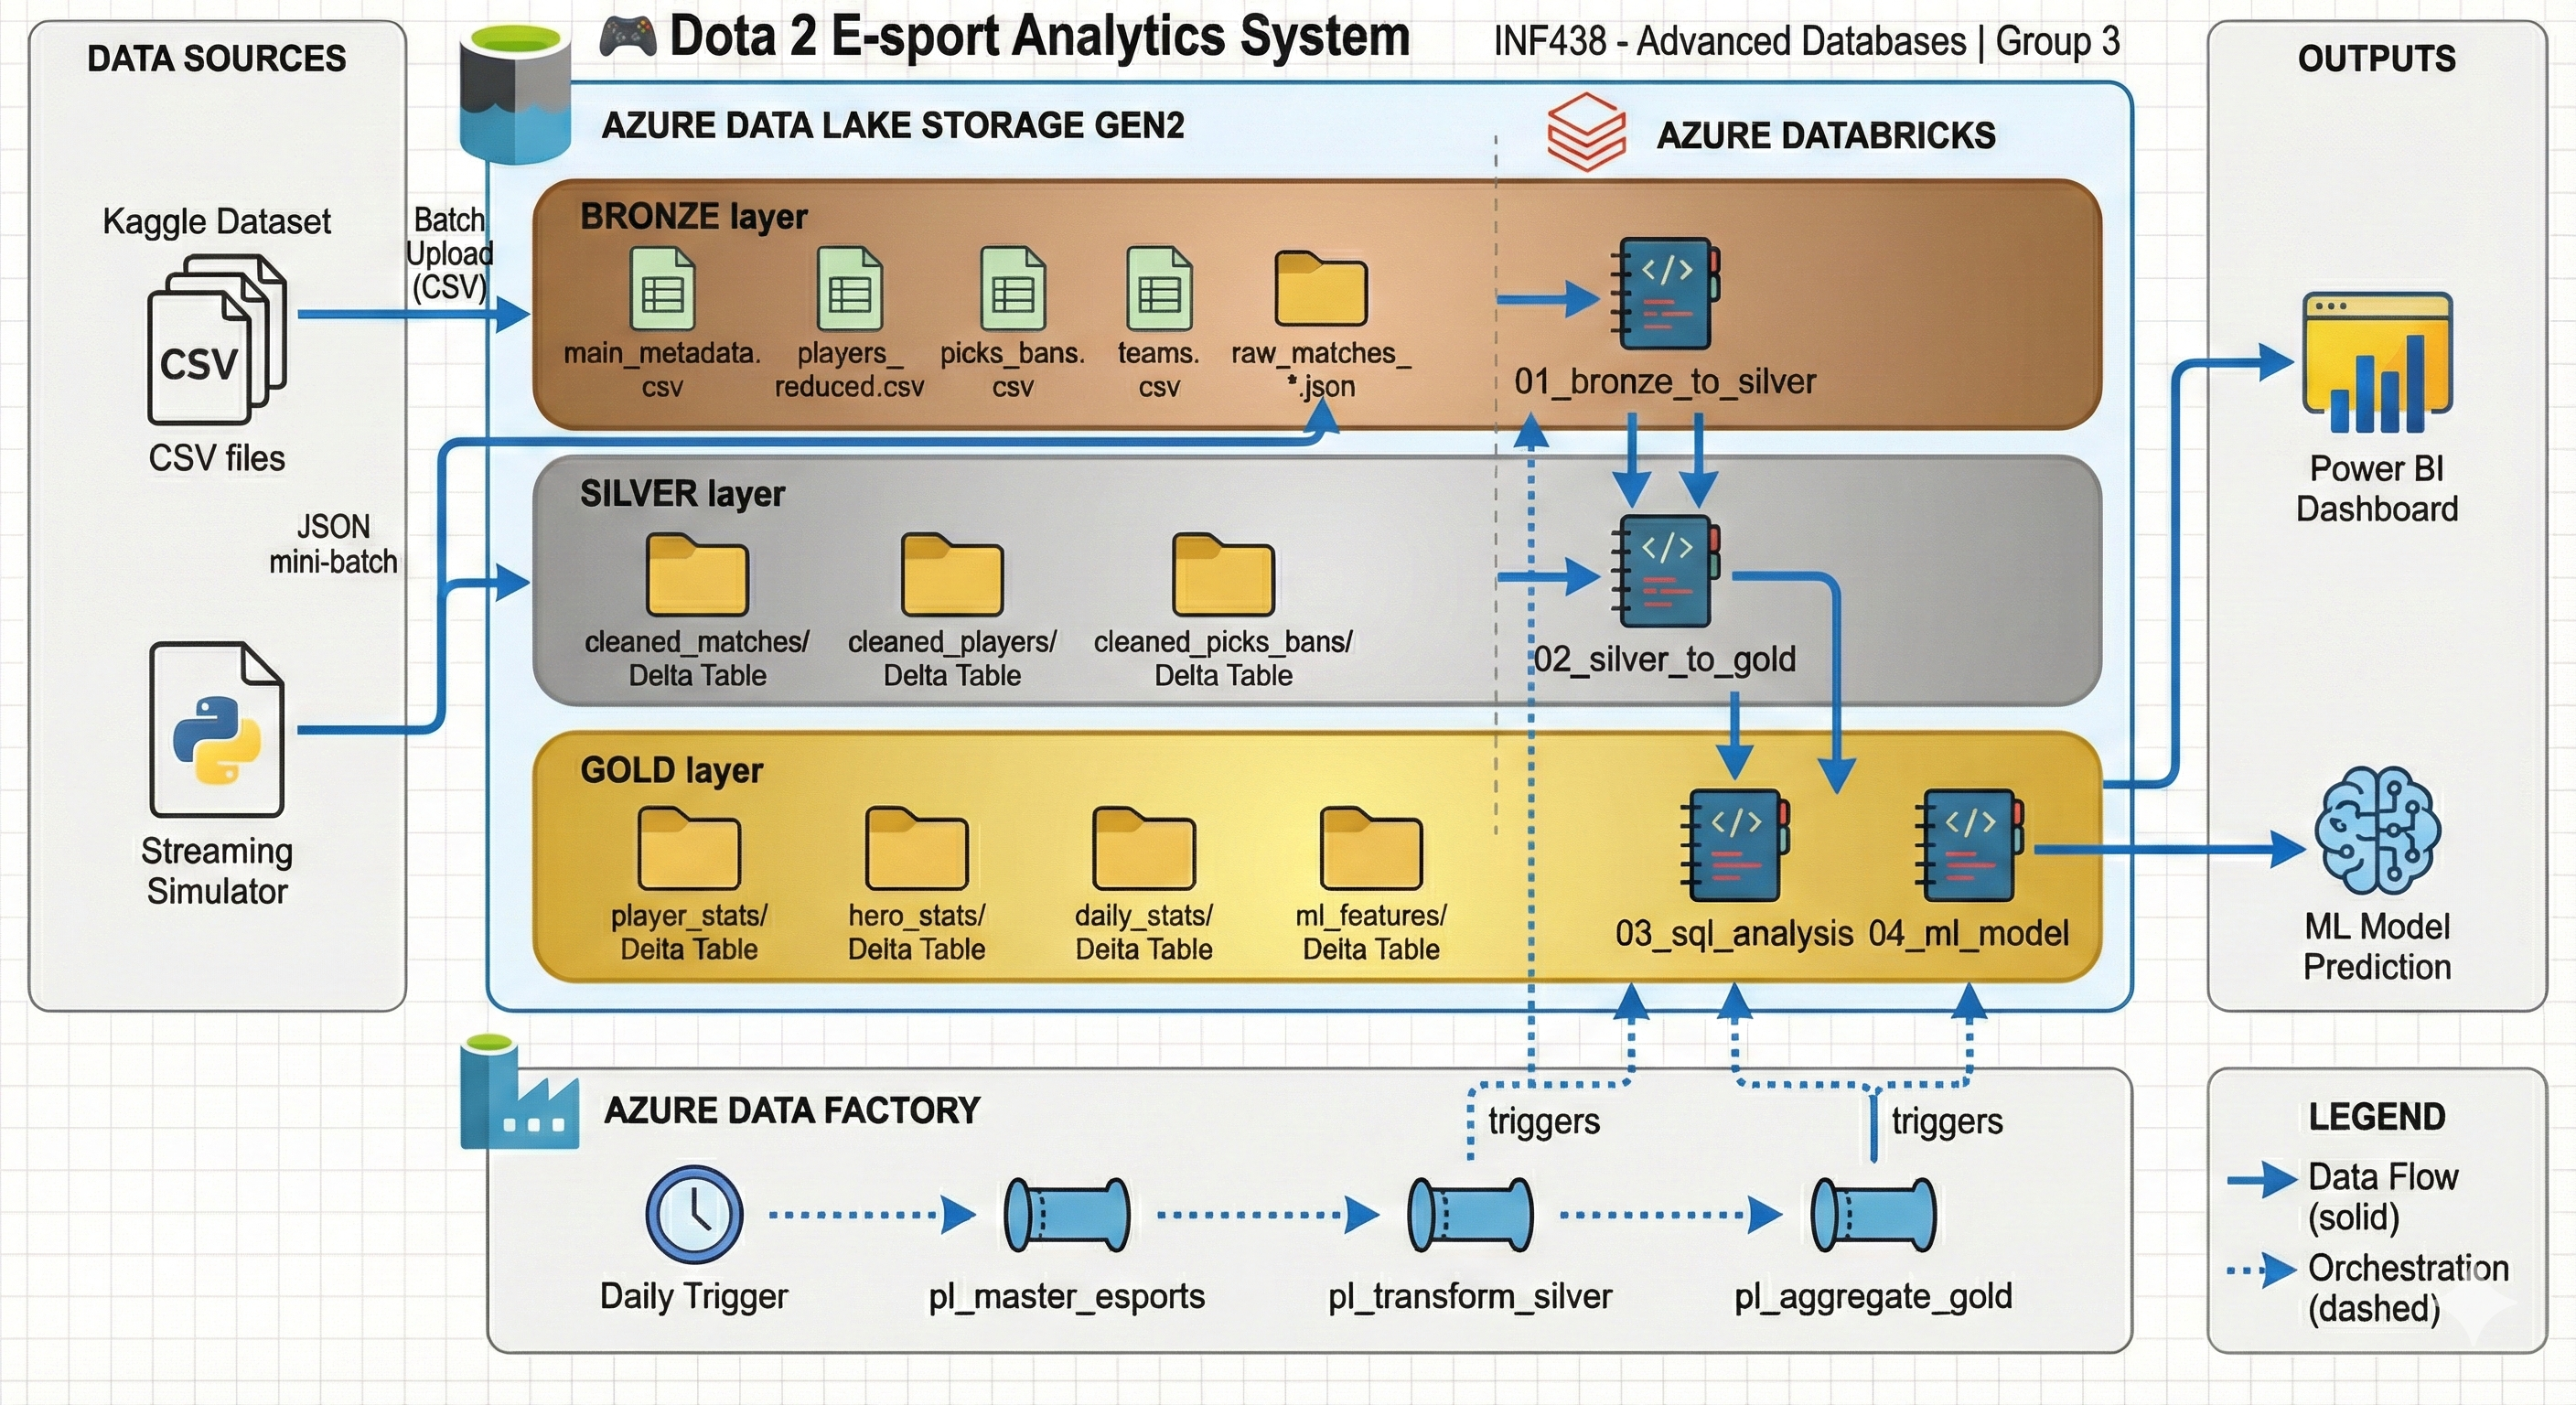
\includegraphics[width=0.60\linewidth]{../Screenshots/pipeline.png}
    \caption{Veri akış diyagramı}
    \label{fig:placeholder}
\end{figure}

% Section 3: Implémentation
\section{Uygulama}

\subsection{Batch İşleme Pipeline'ı}

Batch işleme pipeline orkestrasyonu için Azure Data Factory (ADF) kullanılmıştır. Projede oluşturulan ana pipeline \textbf{pl\_master\_esports} adını taşımaktadır.

Bu işlemin yukarı akışında, \\\texttt{PL\_Ingest\_Kaggle\_To\_Bronze} adlı özel bir veri alma pipeline'ı kurulmuştur. Bu pipeline, ham dosyaları (CSV) ve azaltılmış veri setini Data Lake'in \texttt{bronze/} konteynerine otomatik olarak aktarmak için bir \textit{Copy Data} aktivitesi kullanarak Databricks notebook'ları için veri kullanılabilirliğini sağlar.

\begin{figure}[H]
\centering
\includegraphics[width=\textwidth, height=0.75\textheight, keepaspectratio]{../Screenshots/batch_pipeline.png}
\caption{4 kaynak dosyanın (212 MB) Bronze konteynerine başarılı bir şekilde alındığını onaylayan \textit{Copy Data} aktivitesinin yürütme detayları.}
\label{fig:adf-pipeline}
\end{figure}

Pipeline yapısı aşağıdaki gibi tasarlanmıştır:
\begin{itemize}
    \item \textbf{Aktivite 1:} nb\_bronze\_to\_silver (Databricks Notebook)
    \item \textbf{Aktivite 2:} nb\_silver\_to\_gold (Aktivite 1'e bağlı)
    \item \textbf{Aktivite 3:} nb\_ml\_model (Aktivite 2'ye bağlı)
\end{itemize}

\begin{figure}[H]
\centering
\includegraphics[width=\textwidth, height=0.75\textheight, keepaspectratio]{../Screenshots/Picture3}
\caption{Azure Data Factory'de pl\_master\_esports pipeline diyagramı}
\label{fig:adf-pipeline}
\end{figure}

\subsection{Tetikleyici Yapılandırması}

Otomatik pipeline yürütmesi için \textbf{tr\_daily\_esports} adlı bir tetikleyici oluşturulmuştur.

\begin{table}[H]
\centering
\caption{Tetikleyici yapılandırması}
\label{tab:trigger-config}
\begin{tabular}{>{\centering\arraybackslash}m{4cm}>{\centering\arraybackslash}m{5cm}}
\toprule
\textbf{Parametre} & \textbf{Değer} \\
\midrule
Tetikleyici Adı & tr\_daily\_esports \\
Tip & Schedule Trigger \\
Frekans & Günlük (Daily) \\
Başlangıç Saati & 02:00 UTC \\
Durum & Aktif \\
\bottomrule
\end{tabular}
\end{table}

\begin{figure}[H]
\centering
\includegraphics[width=\textwidth, height=0.75\textheight, keepaspectratio]{../Screenshots/Picture4}
\caption{ADF Monitor ekranında ``Succeeded'' durumu ve ``Triggered by tr\_daily\_esports'' mesajı}
\label{fig:adf-monitor}
\end{figure}

\subsection{Databricks Notebook'ları}

Veri dönüştürme işlemleri Azure Databricks üzerinde PySpark kullanılarak gerçekleştirilmiştir.

\begin{table}[H]
\centering
\caption{Databricks küme yapılandırması}
\label{tab:cluster-config}
\begin{tabular}{>{\centering\arraybackslash}m{4cm}>{\centering\arraybackslash}m{5cm}}
\toprule
\textbf{Parametre} & \textbf{Değer} \\
\midrule
Küme Modu & Standard \\
Node Tipi & Standard\_DS3\_v2 \\
Otomatik Sonlandırma & 120 dakika \\
Databricks Runtime & 13.3 LTS (Spark 3.4.1) \\
\bottomrule
\end{tabular}
\end{table}

\textbf{Oluşturulan Notebook'lar:}
\begin{enumerate}
    \item \textbf{setup\_connection.ipynb} : Azure ADLS Gen2 bağlantı testi
    \item \textbf{01\_bronze\_to\_silver.ipynb} : Ham veri temizleme
    \item \textbf{02\_silver\_to\_gold.ipynb} : İş mantığı uygulaması
    \item \textbf{04\_ml\_model.ipynb} : ML model eğitimi
\end{enumerate}

Bu notebook'ların tam kaynak kodu \textbf{Ek~\ref{appendix:notebooks}}'te mevcuttur.

\subsection{Streaming Simülasyonu}

Gerçek zamanlı bir veri kaynağı olmadığından, streaming davranışını simüle eden bir Python betiği geliştirilmiştir. \textbf{stream\_simulator.py} betiği aşağıdaki mantığa göre çalışır:

\begin{enumerate}
    \item Kayıtlar main\_metadata.csv dosyasından okunur
    \item Kayıtlar 5'li mini-batch'lere bölünür
    \item Her mini-batch için 3 saniyelik yapay bir gecikme uygulanır
    \item Mini-batch benzersiz bir zaman damgası ile adlandırılır ve Bronze'a yazılır
\end{enumerate}

\begin{figure}[H]
\centering
\includegraphics[width=\textwidth, height=0.75\textheight, keepaspectratio]{../Screenshots/simulation-streaming.png}
\caption{stream\_simulator.py yürütme çıktısı}
\label{fig:stream-output}
\end{figure}

Simülatör çalıştırıldığında, Bronze katmanında \texttt{raw\_matches\_YYYYMMDD\_HHMMSS.json} formatında dosyalar oluşturulur (toplamda 10 dosya).

Simülatörün tam kaynak kodu \textbf{Ek~\ref{appendix:streaming}}'te mevcuttur.

\subsection{ETL Dönüşümleri}

\subsubsection{Bronze → Silver Dönüşümü}

Bronze katmanındaki ham CSV verileri kapsamlı bir dönüşüm sürecinden geçmiştir:

\begin{itemize}
    \item \textbf{Yükleme:} Şema çıkarımı ile CSV dosyalarının okunması
    \item \textbf{Temizleme:} Gereksiz sütunların kaldırılması, null değerlerin filtrelenmesi
    \item \textbf{Doğrulama:} Geçersiz süreye ($<$5 dk veya $>$2 saat) sahip maçların filtrelenmesi
    \item \textbf{Zenginleştirme:} Yeni özelliklerin oluşturulması (duration\_minutes, kda\_calculated)
    \item \textbf{Aykırı Değer Tespiti:} 3-sigma kuralı kullanılarak işaretleme
\end{itemize}

\subsubsection{Silver → Gold Dönüşümü}

Temizlenmiş veriler iş mantığı ve gelişmiş hesaplamalar almıştır.

\textbf{Oyuncu İstatistikleri (player\_stats):} Ortalamalar (KDA, GPM, XPM) ve kazanma oranı hesaplaması ile oyuncu hesabına göre toplama. Sonuç: \textbf{813 benzersiz oyuncu} için hesaplanan istatistikler.

\textbf{Kahraman Meta Analizi (hero\_stats):} Kahramanları varlık oranlarına göre 5 katmana sınıflandıran bir algoritma (Tablo~\ref{tab:tier-criteria}'ye bakınız).

\begin{table}[H]
\centering
\caption{Meta Tier sınıflandırma kriterleri}
\label{tab:tier-criteria}
\begin{tabular}{>{\centering\arraybackslash}m{3cm}>{\centering\arraybackslash}m{5cm}}
\toprule
\textbf{Tier} & \textbf{Varlık Oranı Kriteri} \\
\midrule
S-Tier & $>$ 50\% \\
A-Tier & $>$ 30\% \\
B-Tier & $>$ 15\% \\
C-Tier & $>$ 5\% \\
D-Tier & $\leq$ 5\% \\
\bottomrule
\end{tabular}
\end{table}

\begin{figure}[H]
\centering
\includegraphics[width=\textwidth, height=0.75\textheight, keepaspectratio]{../Screenshots/Picture6}
\caption{silver\_to\_gold notebook'unda Tier sınıflandırma çıktısı}
\label{fig:tier-classification}
\end{figure}

\textbf{Maç Süresi Analizi:}

\begin{table}[H]
\centering
\caption{Süre analizi sonuçları}
\label{tab:duration-analysis}
\begin{tabular}{>{\centering\arraybackslash}m{3.5cm}>{\centering\arraybackslash}m{2cm}>{\centering\arraybackslash}m{2cm}>{\centering\arraybackslash}m{2.5cm}}
\toprule
\textbf{Süre} & \textbf{Maçlar} & \textbf{Ort Öldürme} & \textbf{Radiant Kazanma} \\
\midrule
Çok Kısa ($<$25dk) & 4 176 & 44.94 & 53.54\% \\
Kısa (25-35dk) & 13 548 & 56.74 & 50.41\% \\
Orta (35-45dk) & 8 162 & 65.33 & 49.36\% \\
Uzun (45-55dk) & 2 839 & 68.19 & 49.52\% \\
Çok Uzun ($>$55dk) & 1 084 & 80.77 & 50.46\% \\
\bottomrule
\end{tabular}
\end{table}

\subsection{Delta Lake Tablo Yönetimi}

Gold katmanı tabloları Databricks Unity Catalog'da \textbf{esports\_gold} şeması altında yönetilmektedir. SQL oluşturma komutları \textbf{Ek~\ref{appendix:sql}}'de mevcuttur.

\begin{figure}[H]
\centering
\includegraphics[width=\textwidth, height=0.75\textheight, keepaspectratio]{../Screenshots/Picture7}
\caption{Databricks Catalog'da esports\_gold şeması altındaki tabloların listesi}
\label{fig:catalog-tables}
\end{figure}

% Section 4: Analyse et ML
\section{Veri Analizi ve Makine Öğrenmesi}

\subsection{Gold Tablolarına Erişim ve SQL Çalıştırma (Databricks)}

\subsubsection{Azure Data Lake Storage'a Bağlantı (ADLS Gen2)}

\textit{Gold} katmanının analitik tabloları Azure Data Lake Storage Gen2 üzerinde Delta Lake formatında saklanmaktadır.
Bizim durumumuzda, \textit{Azure for Students} aboneliğinin belirli sınırlamaları (kotalar / RBAC izinleri) grup üyelerinin tümü için doğrudan ve istikrarlı erişimi engellemiştir.
Projenin sürekliliğini sağlamak için, \textit{Storage Account}a erişim, gerekli izinlere sahip bir grup üyesi tarafından sağlanan bir erişim anahtarı aracılığıyla yapılmıştır.
Bu anahtar raporda veya sürüm kontrol edilmiş kodda asla açık metin olarak gösterilmez; Databricks ortam değişkenleri aracılığıyla enjekte edilir.

\paragraph{CPU kısıtlamaları ve paylaşılan küme kullanımı.}
Azure for Students aboneliği ile notebook çalıştırma sırasında, bazı Spark işlemelerini kesintiye uğratabilecek kaynak sınırlamalarıyla (CPU/vCore kotası) ve yavaşlamalarla karşılaştık.
Kilitlenmeleri önlemek ve işi zamanında tamamlamak için, bir grup üyesi tarafından önceden yapılandırılmış (esports-cluster) ve daha istikrarlı kaynaklara sahip (16 GB RAM ve 4 çekirdek) Databricks kümesini kullandık.
Bu çözüm sayesinde, ETL dönüşümlerini doğru şekilde yürütebild

ik, Gold katmanındaki Delta tablolarına erişebildik ve analitik SQL sorgularını kesintisiz çalıştırabildik.



\subsubsection{Gold Tablolarının Yüklenmesi ve Geçici Görünümlerin Oluşturulması}

Gold katmanındaki Delta dosyalarında doğrudan SQL sorguları çalıştırmak için, her tabloyu ADLS'den yükledik ve Databricks'te geçici görünümler oluşturduk.

\begin{figure}[H]
\centering
\includegraphics[width=\textwidth]{../Screenshots/gold_tables_created.png}
\caption{ADLS Gen2'den Gold tablolarının yüklenmesi ve Databricks'te geçici görünümlerin oluşturulması}
\label{fig:gold-tables-created}
\end{figure}

\subsection{Analitik SQL Sorguları (Sonuçlar)}

Bu bölüm, oyuncular, kahramanlar ve günlük aktivite üzerine analizler üretmek için kullanılan ana SQL sorgularını sunmaktadır.
Raporun okunabilir kalması için burada çıktıları (ekran görüntüleri) sunuyoruz; tam sorgular gerekirse ekte eklenebilir.

\subsubsection{Performansa Göre İlk 10 Oyuncu (KDA)}

Amaç: Ortalama KDA'larına göre en başarılı 10 oyuncuyu belirlemek (temsili olmayan durumları önlemek için filtreleme ile).

\begin{figure}[H]
\centering
\includegraphics[width=\textwidth]{../Screenshots/player_top10_avg_kda_total_kills_deaths_assists.png}
\caption{SQL Sonucu: Ortalama KDA'ya göre ilk 10 oyuncu (kills, deaths, assists ile)}
\label{fig:sql-top10-players-kda}
\end{figure}

\subsubsection{Günlük Eğilimler: Maç Hacmi ve Ortalama Süre}

Amaç: Maç sayısının günlük evrimini ve ortalama süreyi (dakikaya dönüştürme) gözlemlemek.

\begin{figure}[H]
\centering
\includegraphics[width=\textwidth]{../Screenshots/Last10DaysSummary.png}
\caption{SQL Sonucu: Günlük istatistiklere genel bakış (match\_count ve dakika cinsinden ortalama süre)}
\label{fig:sql-daily-trends}
\end{figure}

\subsubsection{İlk 10 Kahraman: Ekonomik Performans (GPM/XPM)}

Amaç: \texttt{avg\_gpm} ve \texttt{avg\_xpm} üzerinden en iyi ekonomik performansa sahip kahramanları belirlemek.

\begin{figure}[H]
\centering
\includegraphics[width=\textwidth]{../Screenshots/hero_top10_avg_gpm_avg_xpm.png}
\caption{SQL Sonucu: Ortalama GPM ve XPM'ye göre ilk 10 kahraman}
\label{fig:sql-top10-hero-gpm-xpm}
\end{figure}

\subsubsection{İlk 10 Kahraman: Savaş Stili (Öldürme/Asist)}

Amaç: Hacmi (\texttt{times\_played}) dikkate alarak \texttt{avg\_kills} ve \texttt{avg\_assists} metrikleri üzerinden en agresif kahramanları analiz etmek.

\begin{figure}[H]
\centering
\includegraphics[width=\textwidth]{../Screenshots/hero_top10_avg_kills_avg_assists_times_played.png}
\caption{SQL Sonucu: Savaş odaklı ilk 10 kahraman (kills/assists) ve oynanan oyun sayısı}
\label{fig:sql-top10-hero-combat}
\end{figure}

\subsubsection{En Popüler İlk 10 Kahraman}

Amaç: Görülme sayısına (times played) göre en çok oynanan kahramanları belirlemek.
Ayrıca galibiyet sayısını ve galibiyet oranını (\%) da gösteriyoruz.

\begin{figure}[H]
\centering
\includegraphics[width=\textwidth]{../Screenshots/Top10Kahraman.png}
\caption{SQL Sonucu: times\_played'e göre en popüler ilk 10 kahraman (wins ve win\_rate ile)}
\label{fig:sql-top10-heroes-picks}
\end{figure}


Analiz, çok kısa maçlarda ($<$25 dk) Radiant takımının hafif bir avantaja sahip olduğunu (53.54\%) ortaya koymaktadır. Bu oran daha uzun maçlarda %50 civarında dengelenir.

\subsection{Power BI Görselleştirmesi}
\subsubsection{Power BI'da Bağlantı ve Veri Yükleme}

Görselleştirme kısmı, Gold verileri kullanılarak Power BI Desktop ile gerçekleştirilmiştir.
Verileri almak için "Get Data" ve ardından Azure Blob Storage kaynağı kullanılmıştır.
Herkes kolayca bağlantı kuramadığı için (Azure for Students izin/kota sınırlamaları), bir grup üyesi tarafından paylaşılan erişim anahtarı kullanılmıştır.

Bağlantı sağlandıktan sonra, data konteynerindeki (Gold katmanı) Parquet dosyaları bulunmuş ve daily\_stats, player\_stats, hero\_stats ve ml\_features tabloları içe aktarılmıştır.
Ardından, zamana göre filtreleme yapmak için bir Date tablosu eklenmiş ve match\_date sütunu ile daily\_stats tablosuna bağlanmıştır. Son olarak, genel eğilimleri, en iyi oyuncuları ve kahraman metasını analiz etmek için sayfalar ve grafikler oluşturulmuştur.


\subsubsection{Sayfa 1: Genel Bakış ve Günlük Eğilimler}

Bu sayfa 2023 aktivitesinin hızlı bir okumasını sağlar:
(i) tüm göstergeleri kontrol eden bir tarih dilimleyici,
(ii) maç sayısının günlük eğilimi,
(iii) KPI kartları: toplam maç sayısı, ortalama Radiant kazanma oranı ve ortalama maç süresi.

\textbf{Gözlemler.}
Yılın büyük bir bölümünde günlük dalgalanmalarla birlikte nispeten istikrarlı bir aktivite gözlemliyoruz.
Belirli bir dönemde (yıl sonu) belirgin bir zirve görünür, bu bir olaya (turnuva, büyük yama veya yüksek rekabetçi aktivite) karşılık gelebilir.
Ortalama Radiant kazanma oranı dengeye yakın kalır, bu da yıl boyunca kalıcı sistematik bir avantajın olmadığını gösterir.
Ortalama maç süresi genel olarak istikrarlıdır, oyun stili veya meta değişikliklerini gösteren ara sıra varyasyonlarla.

\begin{figure}[H]
\centering
\includegraphics[width=\textwidth]{../Screenshots/pbi_overview_daily_trends.png}
\caption{Power BI --- Genel Bakış Sayfası: zamansal filtre, maç sayısının günlük eğilimi ve global KPI'ler}
\label{fig:pbi-overview}
\end{figure}

\subsubsection{Sayfa 2: İlk 10 Oyuncu}

Bu sayfa oyuncuları şunlara göre karşılaştırır:
(i) Ortalama KDA'ya göre ilk 10 oyuncu,
(ii) Kazanma oranına göre ilk 10 oyuncu,
istatistiklerin detaylı bir tablosu ile (maçlar, kazanmalar, KDA, XPM, vb.).

\textbf{Gözlemler.}
KDA sıralaması bireysel performansa yönelik profilleri vurgular (hayatta kalma + savaş verimliliği).
Kazanma oranı sıralaması mutlaka aynı değildir: bir oyuncu yüksek KDA'ya sahip olabilir ancak daha ılımlı bir kazanma oranına sahip olabilir, bu da takım çalışmasının ve maç bağlamının önemini vurgular.
Tablo, maç hacmini ve göstergeleri eşzamanlı olarak karşılaştırarak sonuçların tutarlılığını doğrulamaya ve çok az maçı olan oyuncuları aşırı yorumlamaktan kaçınmaya olanak tanır.

\begin{figure}[H]
\centering
\includegraphics[width=\textwidth]{../Screenshots/pbi_top10_players.png}
\caption{Power BI --- İlk 10 Oyuncu Sayfası: ortalama KDA vs kazanma oranı karşılaştırması ve detay tablosu}
\label{fig:pbi-top10-players}
\end{figure}

\subsubsection{Sayfa 3: Kahraman Meta Analizi}

Bu sayfa metaya ayrılmıştır:
(i) kahraman başına \textit{presence\_rate} ve \textit{win\_rate}'i ilişkilendiren bir dağılım grafiği,
(ii) en çok bulunan kahramanların ilk 10'u.

\textbf{Gözlemler.}
Dağılım grafiği birkaç ilginç bölgeyi vurgular:
\begin{itemize}
  \item çok mevcut ancak ortalama kazanma oranına sahip kahramanlar: genellikle "meta" veya esnek seçimler, mutlaka baskın değil;
  \item az mevcut ancak yüksek kazanma oranına sahip kahramanlar: "underrated" adaylar veya çok etkili durumsal seçimler;
  \item mevcut ve performanslı kahramanlar: baskın metayı oluştururlar ve özel dikkat hak ederler.
\end{itemize}
En çok bulunan kahramanların ilk 10'u popülariteyi sentezler ve filtrelenen dönemde en sık oynanan kahramanların tanımlanmasını kolaylaştırır.

\begin{figure}[H]
\centering
\includegraphics[width=\textwidth]{../Screenshots/pbi_hero_meta.png}
\caption{Power BI --- Kahraman Meta Sayfası: presence rate vs win rate ilişkisi ve en çok bulunan kahramanların ilk 10'u}
\label{fig:pbi-hero-meta}
\end{figure}

\subsubsection{Sayfa 4: Maç Süresi ve Korelasyonlar}

Bu sayfa şunları analiz eder:
(i) ortalama maç süresinin zamansal evrimi,
(ii) bir dağılım grafiği aracılığıyla süre ve yoğunluk (örn. ortalama öldürmeler) arasındaki ilişki.

\textbf{Gözlemler.}
Ortalama süre nispeten sınırlı bir aralıkta değişir, ancak bazı çukurlar/zirveler maçların daha hızlı bittiği (agresif stratejiler) veya tersine uzadığı (daha kontrollü oyunlar) dönemleri önerir.
Süre vs öldürmeler dağılım grafiği genel olarak zayıf ila orta bir ilişki gösterir: daha uzun maçlar daha fazla savaş fırsatı sunma eğilimindedir, ancak dağılım diğer faktörlerin öldürme sayısını güçlü bir şekilde etkilediğini gösterir (seviye farkı, draft'lar, takım stilleri).
Bu grafik bu nedenle mükemmel doğrusal bir ilişkinin olmadığını, daha çok genel bir eğilim olduğunu doğrulamaya yarar.

\begin{figure}[H]
\centering
\includegraphics[width=\textwidth]{../Screenshots/pbi_duration_correlation.png}
\caption{Power BI --- Süre ve Korelasyonlar Sayfası: ortalama süre eğilimi ve süre vs öldürmeler korelasyonu}
\label{fig:pbi-duration-corr}
\end{figure}



\subsection{Makine Öğrenmesi Modeli}

Maç sonucunu tahmin etmek için bir ikili sınıflandırma modeli geliştirilmiştir. Hedef değişken \texttt{win}'dir (1 = Kazanma, 0 = Kaybetme).

\begin{table}[H]
\centering
\caption{Kullanılan Özellikler (Features)}
\label{tab:features}
\begin{tabular}{>{\centering\arraybackslash}m{3.5cm}>{\centering\arraybackslash}m{5cm}>{\centering\arraybackslash}m{3cm}}
\toprule
\textbf{Feature} & \textbf{Açıklama} & \textbf{Kategori} \\
\midrule
kills & Öldürme Sayısı & Savaş \\
deaths & Ölüm Sayısı & Savaş \\
assists & Asist Sayısı & Savaş \\
gold\_per\_min & Dakika başına altın & Ekonomi \\
xp\_per\_min & Dakika başına tecrübe (XP) & Ekonomi \\
hero\_damage & Kahraman hasarı & Hasar \\
tower\_damage & Kule hasarı & Hasar \\
last\_hits & Son vuruş sayısı & İlerleme \\
level & Oyuncu seviyesi & İlerleme \\
duration\_minutes & Maç süresi & Maç Bilgisi \\
\bottomrule
\end{tabular}
\end{table}

\textbf{Random Forest Classifier} algoritması şu parametrelerle seçilmiştir: numTrees=50, maxDepth=10, Train/Test Split=80\%/20\%.

ML pipeline'ının tam kaynak kodu \textbf{Ek~\ref{appendix:ml}}'de mevcuttur.

\subsection{Model Sonuçları}

\begin{center}
\fbox{
\begin{minipage}{0.7\textwidth}
\centering
\vspace{0.5cm}
\textbf{\large MODEL SONUÇLARI}\\[0.5cm]
\rule{0.9\textwidth}{0.5pt}\\[0.3cm]
Kullanılan Model: \textbf{Random Forest Classifier}\\[0.3cm]
Doğruluk (Accuracy): \textbf{\LARGE 87.34\%}\\[0.3cm]
\rule{0.9\textwidth}{0.5pt}
\vspace{0.5cm}
\end{minipage}
}
\end{center}

\begin{table}[H]
\centering
\caption{Karışıklık Matrisi (Confusion Matrix)}
\label{tab:confusion-matrix}
\begin{tabular}{>{\centering\arraybackslash}m{3cm}|>{\centering\arraybackslash}m{2.5cm}>{\centering\arraybackslash}m{2.5cm}}
\toprule
\textbf{Gerçek / Tahmin} & \textbf{Kaybetme (0)} & \textbf{Kazanma (1)} \\
\midrule
\textbf{Kaybetme (0)} & 727 (GN) & 131 (YP) \\
\textbf{Kazanma (1)} & 81 (YN) & 735 (GP) \\
\bottomrule
\end{tabular}
\end{table}

\textbf{Hesaplanan Metrikler :}
\begin{itemize}
    \item Gerçek Pozitif Oranı (Recall) : $\frac{735}{735+81} = 90.07\%$
    \item Gerçek Negatif Oranı : $\frac{727}{727+131} = 84.73\%$
    \item Kesinlik (Precision) : $\frac{735}{735+131} = 84.87\%$
\end{itemize}

\subsection{Özellik Önem Analizi}

\begin{table}[H]
\centering
\caption{Özellik Önem Sıralaması}
\label{tab:feature-importance}
\begin{tabular}{>{\centering\arraybackslash}m{2cm}>{\centering\arraybackslash}m{4cm}>{\centering\arraybackslash}m{4cm}}
\toprule
\textbf{Sıra} & \textbf{Feature} & \textbf{Önem} \\
\midrule
1 & assists & 0.311480 \\
2 & deaths & 0.204537 \\
3 & tower\_damage & 0.147192 \\
4 & xp\_per\_min & 0.073274 \\
5 & last\_hits & 0.058863 \\
6 & duration\_minutes & 0.049268 \\
7 & gold\_per\_min & 0.048150 \\
8 & kills & 0.040887 \\
9 & hero\_damage & 0.040081 \\
10 & level & 0.026267 \\
\bottomrule
\end{tabular}
\end{table}

Bu sonuçlar, \textbf{takım çalışmasının} (0.311 ile \texttt{assists}) maç sonucu üzerinde en belirleyici faktör olduğunu, bunu \textbf{hayatta kalmanın} (0.205 ile \texttt{deaths}) ve \textbf{hedef hasarının} (0.147 ile \texttt{tower\_damage}) izlediğini göstermektedir.

Beklentilerin aksine, ekonomik faktörler (\texttt{gold\_per\_min}: 0.048, \texttt{xp\_per\_min}: 0.073) nispeten düşük öneme sahiptir. Bu, profesyonel Dota 2 maçlarında takım koordinasyonunun ve hedef odaklı oyunun, bireysel kaynak birikiminden daha fazla zafer öngördürücü olduğunu göstermektedir.

\subsection{MLflow Takibi}

Tüm model denemeleri \texttt{mlflow.autolog()} ile MLflow üzerinde otomatik olarak izlenmiştir.

\begin{figure}[H]
\centering
\includegraphics[width=\textwidth, height=0.75\textheight, keepaspectratio]{../Screenshots/Picture9}
\caption{MLflow arayüzünde model sonuçları ve parametreler}
\label{fig:mlflow-results}
\end{figure}

% Section 5: Difficultés et Solutions
\section{Karşılaşılan Zorluklar ve Çözümler}

\subsection{Azure Kaynak Sınırlamaları}

\textbf{Sorun:} Azure for Students aboneliği belirli katı kaynak sınırlamaları içermektedir (özellikle vCore kotası ve sınırlı krediler).

\textbf{Çözüm:} Küme boyutu minimumda tutuldu (Standard\_DS3\_v2), otomatik sonlandırma süresi 120 dakikaya ayarlandı ve küme kredileri biriktirmek için işlemler bittikten sonra manuel olarak durduruldu.

\subsection{Streaming Simülasyonunda Dosya Çakışmaları}

\textbf{Sorun:} Simülasyon betiğinin hızlı çalıştırılması sırasında, aynı saniye içinde birden fazla mini-batch oluşturulabiliyordu, bu da dosya adı çakışmalarına ve veri üzerine yazmaya neden oluyordu.

\textbf{Çözüm:} Veri alma döngüsüne \texttt{SLEEP\_TIME = 3} saniyelik bir gecikme eklendi. Ayrıca, dosya adları artık \texttt{YYYYMMDD\_HHMMSS} formatında kesin bir zaman damgası kullanmaktadır.

\subsection{Veri Hacmi ve Maliyet Kısıtlamaları}

\textbf{Sorun:} Orijinal kaynak dosyası \texttt{players.csv} 5.3 GB'ı aşıyordu. Bu tam hacmin işlenmesi Azure kredilerini ve mevcut öğrenci kümesinin hesaplama kapasitesini hızla tüketecekti.

\textbf{Çözüm:} Temsili bir \texttt{players\_reduced.csv} dosyası (152 MB) oluşturmak için yerel ön işleme yapıldı. Ardından bu azaltılmış veri setinde okuma/yazma performansını optimize etmek için Delta Lake formatı kullandık.

\subsection{Azure Storage Anahtar Yönetimi}

\textbf{Sorun:} Storage account anahtarının, kodda açık metin olarak gösterilmeden geliştiriciler ve hizmetler arasında paylaşılması gerekiyordu.

\textbf{Çözüm:} Ortam değişkenlerinin kullanımı (\texttt{AZURE\_STORAGE\_KEY}), Databricks secrets ile güvenli depolama ve \texttt{.env} dosyası ile yerel geliştirme.

\subsection{Erişim Yönetimi Karmaşıklığı (IAM)}

\textbf{Sorun:} Ekip işbirliği tekrarlayan izin sorunları (IAM) yarattı. "Contributor" rolünün atanması belirli işlemler için (Blob verilerini okuma veya Cost Management'a erişim gibi) yeterli değildi, bu da zaman yönetiminde ve proje ilerlemesinde önemli gecikmelere neden oldu.

\textbf{Çözüm:} Daha ayrıntılı bir RBAC stratejisi benimsendi, uygun üyelere Azure portalı üzerinden açıkça \textit{Storage Blob Data Owner} ve \textit{Cost Management Contributor} rolleri atandı.

\newpage
\subsection{Databricks Cluster Erişim Sorunları}

\textbf{Sorun:} \textit{Azure for Students} aboneliğinin sınırlamaları nedeniyle, bir Databricks kümesi oluşturamıyor veya seçemiyorduk, bu da notebook yürütmesini ve dolayısıyla Gold verileri üzerinde SQL analizlerinin başlatılmasını engelliyordu.

\textbf{Çözüm:} Projenin ilerlemesini sağlamak için, gerekli izinlere sahip bir grup üyesi geçici olarak Databricks kümesine (\textit{esports-cluster}) erişim yetkisi verdi. Bu, Gold tablolarında SQL sorguları yürütmemize ve analitik aşamaya devam etmemize olanak sağladı. Erişim bilgileri açık metin olarak gösterilmedi: anahtar ve bağlantı parametreleri Databricks ortam değişkenleri ve \textit{Databricks Secrets} aracılığıyla güvenli bir şekilde yönetildi.

% Section 6: Conclusion
\section{Sonuç}

\subsection{Proje Özeti}

Bu proje, modern veri mühendisliği kavramlarının (Lakehouse, Delta Lake, MLOps) pratik bir e-spor senaryosunda nasıl uygulanabileceğini göstermiştir.

\begin{table}[H]
\centering
\caption{Elde Edilen Temel Sonuçlar}
\label{tab:results-summary}
\begin{tabular}{>{\centering\arraybackslash}m{4cm}>{\centering\arraybackslash}m{8cm}}
\toprule
\textbf{Bileşen} & \textbf{Sonuç} \\
\midrule
Medallion Mimarisi & Bronze/Silver/Gold katmanları kuruldu \\
Veri İşleme & 29.809 maç, 8.456 oyuncu işlendi \\
Streaming Simülasyonu & Bronze katmanına 10 mini-batch yazıldı \\
Gold Tabloları & 4 analitik tablo (813 oyuncu, 123 kahraman) \\
ML Modeli & \%87.34 doğruluk oranlı Random Forest \\
Meta Analizi & 5 seviyeli kahraman sınıflandırması \\
\bottomrule
\end{tabular}
\end{table}

\subsection{Öğrenilen Dersler}

\begin{itemize}
    \item \textbf{Bulut Kaynak Yönetimi:} Azure maliyet ve kaynak optimizasyonu
    \item \textbf{Delta Lake Avantajları:} ACID işlemleri, şema evrimi, performans
    \item \textbf{Orkestrasyon:} Azure Data Factory ile karmaşık akışları yönetme
    \item \textbf{MLOps Uygulamaları:} MLflow ile deney takibinin önemi
\end{itemize}

\subsection{Genel Sonuç}

Azure ekosistemi tarafından sunulan entegre hizmetler, uçtan uca veri çözümünün hızlı ve verimli geliştirilmesini sağladı. \textbf{\%87.34} doğruluk oranına sahip ML modeli, oyuncu performans metriklerinin maç sonucunu yüksek kesinlikle tahmin edebileceğini kanıtladı. Özellikle, ekonomik faktörler (\texttt{gold\_per\_min}, \texttt{xp\_per\_min}) en belirleyici özellikler olarak tanımlandı.

\newpage
\appendix
\section*{EKLER}
\addcontentsline{toc}{section}{Ekler}

\subsection*{Databricks Notebook Kaynak Kodları}
\label{appendix:notebooks}

\subsubsection*{setup\_connection.ipynb}

\begin{lstlisting}[language=Python, caption=Azure ADLS Gen2 Bağlantı Testi]
# Notebook: setup_connection
import os

storage_account = "dota2lakehousenew"
container = "data"
storage_account_key = os.environ.get("AZURE_STORAGE_KEY")
print(f"Key loaded: {storage_account_key is not None}")

spark.conf.set(
  f"fs.azure.account.key.{storage_account}.dfs.core.windows.net",
  storage_account_key)

BRONZE = f"abfss://{container}@{storage_account}.dfs.core.windows.net/bronze"
SILVER = f"abfss://{container}@{storage_account}.dfs.core.windows.net/silver"
GOLD = f"abfss://{container}@{storage_account}.dfs.core.windows.net/gold"

print("=== Files in Bronze Layer ===")
for f in dbutils.fs.ls(BRONZE):
  print(f"  {f.name} ({f.size/1024/1024:.2f} MB)")
\end{lstlisting}

\subsubsection*{01\_bronze\_to\_silver.ipynb (Extraits)}

\begin{lstlisting}[language=Python, caption=Veri Yükleme ve Temizleme]
from pyspark.sql.functions import *
df_matches = spark.read.csv(f"{BRONZE}/main_metadata.csv",
  header=True, inferSchema=True)
df_players = spark.read.csv(f"{BRONZE}/players_reduced.csv",
  header=True, inferSchema=True)
df_matches_clean = df_matches \
  .drop("Unnamed: 0").dropDuplicates(["match_id"]) \
  .filter(col("match_id").isNotNull()) \
  .filter((col("duration") > 300) & (col("duration") < 7200))
df_matches_clean = df_matches_clean \
  .withColumn("duration_minutes", round(col("duration")/60, 2)) \
  .withColumn("radiant_win", col("radiant_win").cast("boolean")) \
  .withColumn("match_date", to_date(col("start_date_time")))
stats = df_players.select(
  mean("kills").alias("m"), stddev("kills").alias("s")).collect()[0]
df_players = df_players.withColumn("is_outlier",
  when(col("kills") > stats["m"] + 3*stats["s"], True).otherwise(False))
df_matches_clean.write.format("delta").mode("overwrite") \
  .save(f"{SILVER}/cleaned_matches")
\end{lstlisting}

\subsubsection*{02\_silver\_to\_gold.ipynb (Extraits)}

\begin{lstlisting}[language=Python, caption=Gold Tablolarının Oluşturulması]
df_player_stats = df_players \
  .filter(col("account_id").isNotNull()) \
  .groupBy("account_id").agg(
    count("match_id").alias("total_matches"),
    sum("win").alias("total_wins"),
    round(avg("kills"), 2).alias("avg_kills"),
    round(avg("kda_calculated"), 2).alias("avg_kda"),
    round(avg("gold_per_min"), 2).alias("avg_gpm")) \
  .withColumn("win_rate",
    round(col("total_wins")/col("total_matches")*100, 2))
total = df_matches.count()
df_hero = df_hero \
  .withColumn("presence_rate", 
    round(col("total_presence")/(total*2)*100, 2)) \
  .withColumn("meta_tier",
    when(col("presence_rate") > 50, "S-Tier")
    .when(col("presence_rate") > 30, "A-Tier")
    .when(col("presence_rate") > 15, "B-Tier")
    .when(col("presence_rate") > 5, "C-Tier")
    .otherwise("D-Tier"))
\end{lstlisting}

\newpage
\subsection*{Streaming Simülatörü Kaynak Kodu}
\label{appendix:streaming}

\begin{lstlisting}[language=Python, caption=stream\_simulator.py - Streaming Simülatörü]
import time, pandas as pd, os
from datetime import datetime
from azure.storage.filedatalake import DataLakeServiceClient

STORAGE_ACCOUNT = "dota2lakehousenew"
STORAGE_KEY = os.getenv("AZURE_STORAGE_ACCOUNT_KEY")
CONTAINER = "data"
DIRECTORY = "bronze"
SOURCE_FILE = "main_metadata.csv"

def get_client():
  url = f"https://{STORAGE_ACCOUNT}.dfs.core.windows.net"
  return DataLakeServiceClient(account_url=url, credential=STORAGE_KEY)

def stream_data():
  print("--- Starting Streaming Simulation ---")
  df = pd.read_csv(SOURCE_FILE)
  print(f"Loaded {len(df)} rows.")

  client = get_client()
  fs_client = client.get_file_system_client(CONTAINER)
  dir_client = fs_client.get_directory_client(DIRECTORY)

  BATCH_SIZE, SLEEP_TIME = 5, 3

  for i in range(0, 50, BATCH_SIZE):
    chunk = df.iloc[i:i+BATCH_SIZE]
    json_data = chunk.to_json(orient='records')
    
    ts = datetime.now().strftime("%Y%m%d_%H%M%S")
    fname = f"raw_matches_{ts}.json"
    
    fc = dir_client.get_file_client(fname)
    fc.create_file()
    fc.append_data(data=json_data, offset=0, length=len(json_data))
    fc.flush_data(len(json_data))
    print(f"Uploaded {fname}")
    
    time.sleep(SLEEP_TIME)

  print("--- Simulation Complete ---")

if __name__ == "__main__":
  stream_data()
\end{lstlisting}

\newpage
\subsection*{Tablo Oluşturma SQL Komutları}
\label{appendix:sql}

\begin{lstlisting}[language=SQL, caption=Şema ve Gold Tablolarının Oluşturulması]
CREATE DATABASE IF NOT EXISTS esports_gold;
CREATE TABLE IF NOT EXISTS esports_gold.player_stats
USING DELTA LOCATION
  'abfss://data@dota2lakehousenew.dfs.core.windows.net/gold/player_stats';
CREATE TABLE IF NOT EXISTS esports_gold.hero_stats
USING DELTA LOCATION
  'abfss://data@dota2lakehousenew.dfs.core.windows.net/gold/hero_stats';
CREATE TABLE IF NOT EXISTS esports_gold.daily_stats
USING DELTA LOCATION
  'abfss://data@dota2lakehousenew.dfs.core.windows.net/gold/daily_stats';
CREATE TABLE IF NOT EXISTS esports_gold.ml_features
USING DELTA LOCATION
  'abfss://data@dota2lakehousenew.dfs.core.windows.net/gold/ml_features';
SHOW TABLES IN esports_gold;
\end{lstlisting}

\newpage
\subsection*{ML Model Kaynak Kodu}
\label{appendix:ml}

\begin{lstlisting}[language=Python, caption=Tam Makine Öğrenmesi Pipeline'ı]
import mlflow
from pyspark.ml.feature import VectorAssembler
from pyspark.ml.classification import RandomForestClassifier
from pyspark.ml.evaluation import MulticlassClassificationEvaluator
from pyspark.ml import Pipeline
path = f"abfss://{container}@{storage_account}.dfs.core.windows.net/gold/ml_features"
df = spark.read.format("delta").load(path)
cols = ["kills", "deaths", "assists", "gold_per_min", "xp_per_min",
  "hero_damage", "tower_damage", "last_hits", "level",
  "duration_minutes", "win"]
data = df.select(cols).dropna()
train, test = data.randomSplit([0.8, 0.2], seed=42)
features = [c for c in cols if c != "win"]
assembler = VectorAssembler(inputCols=features, outputCol="features")
rf = RandomForestClassifier(
  labelCol="win", featuresCol="features", numTrees=50, maxDepth=10)
pipeline = Pipeline(stages=[assembler, rf])
mlflow.autolog()
model = pipeline.fit(train)
predictions = model.transform(test)
evaluator = MulticlassClassificationEvaluator(
  labelCol="win", predictionCol="prediction", metricName="accuracy")
acc = evaluator.evaluate(predictions)
print(f"Accuracy: {acc*100:.2f}%")

predictions.groupBy("win", "prediction").count().show()
import pandas as pd
imp = model.stages[-1].featureImportances.toArray()
df_imp = pd.DataFrame({"Feature": features, "Importance": imp})
print(df_imp.sort_values("Importance", ascending=False))
\end{lstlisting}

\newpage
\subsection*{Kullanılan Teknolojiler}
\label{appendix:technologies}

\begin{table}[H]
\centering
\caption{Proje Teknoloji Yığını}
\begin{tabular}{>{\centering\arraybackslash}m{4cm}>{\centering\arraybackslash}m{4cm}>{\centering\arraybackslash}m{3cm}}
\toprule
\textbf{Kategori} & \textbf{Teknoloji} & \textbf{Sürüm} \\
\midrule
Bulut Platformu & Microsoft Azure & - \\
Storage Account & dota2lakehousenew & ADLS Gen2 \\
Orkestrasyon & Azure Data Factory & V2 \\
İşlem & Azure Databricks & 13.3 LTS \\
İşleme & Apache Spark & 3.4.1 \\
Dil & Python / PySpark & 3.10 \\
Veri Formatı & Delta Lake & 2.4.0 \\
ML Takibi & MLflow & Otomatik \\
Görselleştirme & Power BI & - \\
\bottomrule
\end{tabular}
\end{table}

\end{document}